\subsection{与正合列相伴的类}

命题 1. --- 设 (C, d) 和 (C', d') 为两个左 A-模复形，n、p、q 为三个整数，使得 \(p \geqslant q\) 。对于 \(p \geqslant i \geqslant q - 1\) ，设 \(f_i: C_i \to C_{i+n+1}'\) 为一个 A-模同态，使得 \(f_p \circ d = 0\) ， \(f_i \circ d = d' \circ f_{i+1}\) （当 \(p > i \geqslant q - 1\) ），且 \(d' \circ f_{q-1} = 0\) （见图 2）。

\pandocbounded{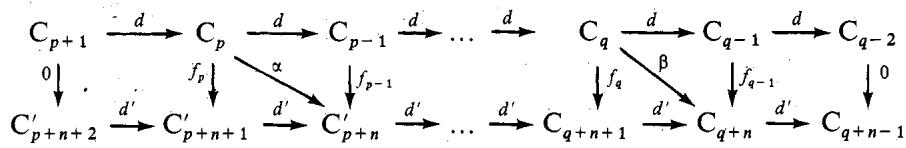
\includegraphics[keepaspectratio]{images/part001_b19b44e0.jpg}}\\
图 2。

令 \(\alpha = f_{p-1} \circ d = d' \circ f_p\) , \(\beta = f_{q-1} \circ d = d' \circ f_q\) ，并设 \(a\) (相应地， \(b\) )为从 C 到 C' 的度为 \(n\) 的分次 A-同态，其仅有的非零双齐次分量是 \(\alpha\) (相应地， \(\beta\) )。则有 \(a \in Z_n(\text{Homgr}_A(C, C'))\) , \(b \in Z_n(\text{Homgr}_A(C, C'))\) 和 \(a - (-1)^{(n+1)(p-q)} b \in B_n(\text{Homgr}_A(C, C'))\) 。

我们有 \(d' \circ \alpha = d' \circ d' \circ f_p = 0\) , \(\alpha \circ d = f_{p-1} \circ d \circ d = 0\) ，因此

\[
a \in Z _ {n} \left(\operatorname{Homgr} _ {\mathrm{A}} \left(\mathrm{C}, \mathrm{C} ^ {\prime}\right)\right);
\]

同理 \(b \in Z_n(\text{Homgr}_A(C, C'))\) 。令 \(\varepsilon = (-1)^{n+1}\) 。在复形 \(\text{Homgr}_A(C, C')\) 中有以下关系

\[
\mathrm{D} f _ {p - 1} = d ^ {\prime} \circ f _ {p - 1} - \varepsilon f _ {p - 1} \circ d = f _ {p - 2} \circ d - \varepsilon \alpha
\]

\[
\mathrm{D} f _ {i} = d ^ {\prime} \circ f _ {i} - \varepsilon f _ {i} \circ d = f _ {i - 1} \circ d - \varepsilon f _ {i} \circ d (p - 1 > i > q)
\]

\[
\mathrm{D} f _ {q} = d ^ {\prime} \circ f _ {q} - \varepsilon f _ {q} \circ d = \beta - \varepsilon f _ {q} \circ d,
\]

因此

\[
\sum_ {i = 1} ^ {p - q} \varepsilon^ {i} D f _ {p - i} = \varepsilon^ {p - q} \beta - \alpha ,
\]

这便证明了引理。

考虑两个左 A-模 M 与 N，以及一个 A-模正合列

\[
0 \rightarrow \mathrm{N} \rightarrow \mathrm{R} _ {n} \rightarrow \mathrm{R} _ {n - 1} \rightarrow \dots \rightarrow \mathrm{R} _ {1} \rightarrow \mathrm{M} \rightarrow 0.\tag{4}
\]

根据 X 第 49 页的命题 3 与命题 3 bis，存在一个交换图：

\begin{enumerate}
\def\labelenumi{(\arabic{enumi})}
\setcounter{enumi}{4}
\tightlist
\item
\end{enumerate}

\pandocbounded{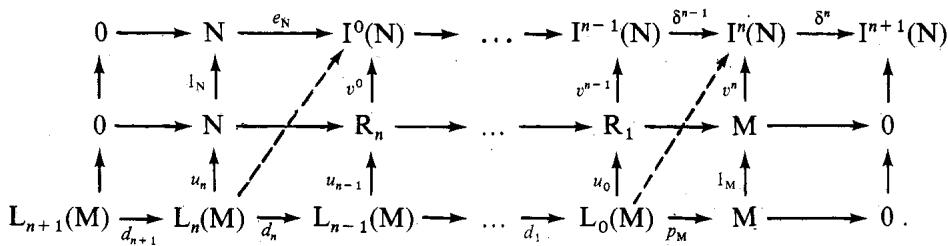
\includegraphics[keepaspectratio]{images/part001_efe78803.jpg}}

考虑这两个元素 \(b\) 与 \(a\) （它们属于 \(\mathrm{Homgr}_{\mathbf{A}}(\mathrm{L}(\mathbf{M}),\mathrm{I}(\mathbf{N}))\) ），其仅有的非零双齐次分量分别是

\[
b ^ {n} = e _ {\mathrm{N}} \circ u _ {n}: \mathrm{L} _ {n} (\mathrm{M}) \rightarrow \mathrm{I} ^ {0} (\mathrm{N}) \quad \text { and } \quad a ^ {n} = v ^ {n} \circ p _ {\mathrm{M}}: \mathrm{L} _ {0} (\mathrm{M}) \rightarrow \mathrm{I} ^ {n} (\mathrm{N})
\]

分别。

命题 2. --- 有 \(a\) , \(b \in Z^n(\text{Homgr}_A (\text{L(M)}, \text{l(N)})\) ）。此外，类 \(\overline{a}\) 与 \(\overline{b}\) ——即 \(a\) 与 \(b\) 的类——在 \(\text{H}^n(\text{Homgr}_A (\text{L(M)}, \text{l(N)})) = \text{Ext}_A^n (\text{M}, \text{N})\) 中仅依赖于正合列 (4)，并且相等。

将命题 1 应用于 (5) 中两端的行以及复合的竖直箭头，取 \(p = n\) , \(q = 0\) ，则有 \(a\) , \(b \in \mathbf{Z}^{n}(\mathrm{Homgr}_{\mathrm{A}}(\mathrm{l(M)}, \mathrm{L(N)}))\) ，并且

\[
a - b = a - (- 1) ^ {(n + 1) n} b \in \mathrm{B} ^ {n} (\operatorname{Homgr} _ {\mathrm{A}} (\mathrm{L} (\mathrm{M}), \mathrm{I} (\mathrm{N}))).
\]

由于 \(a\) （相应地， \(b\) ）与 \(u\) （相应地， \(v\) ）的选取无关，元素 \(\overline{a} = \overline{b}\) （属于 \(\mathrm{Ext}_{\mathbf{A}}^{n}\) (M, N)）与态射 \(u\) 和 \(v\) 的选取无关，由此得出该命题。

定义 1. --- 元素 \(\theta\) ，即 \(\operatorname{Ext}_{\mathbf{A}}^{n}(\mathbf{M}, \mathbf{N})\) 中由 \(\theta = (-1)^{n(n+1)/2} \overline{a} = (-1)^{n(n+1)/2} \overline{b}\) 所定义的元素，称为与正合列 (4) 相伴的类。

注记. --- 1) 设 (P, p) 是 M 的一个投射分解。由 X 第 49 页命题 3，存在一个交换图

\[
\begin{array}{c} 0 \longrightarrow \mathrm{N} \longrightarrow \mathrm{R} _ {n} \longrightarrow \dots \longrightarrow \mathrm{R} _ {1} \longrightarrow \mathrm{M} \longrightarrow 0 \\ \tilde {u} _ {n} \uparrow \quad \tilde {u} _ {n - 1} \uparrow \quad \tilde {u} _ {0} \uparrow \quad \uparrow_ {\mathrm{M}} \\ \mathrm{P} _ {n} \longrightarrow \mathrm{P} _ {n - 1} \longrightarrow \dots \longrightarrow \mathrm{P} _ {0} \xrightarrow {p} \mathrm{M} \longrightarrow 0. \end{array}
\]

使用 § 6 的记号，θ 是态射 P → N 的同伦类在 φ(P, N) 下的像，该态射由 \((-1)^{n(n+1)/2} \tilde{u}_{n}\) 定义。类似地，若 \((e, E)\) 是 N 的一个内射分解，则存在一个交换图

\[
\begin{array}{c} 0 \longrightarrow \mathrm{N} \longrightarrow \mathrm{E} ^ {0} \longrightarrow \dots \longrightarrow \mathrm{E} ^ {n - 1} \longrightarrow \mathrm{E} ^ {n} \\ 1 _ {\mathrm{N}} \uparrow \quad \tilde {v} ^ {0} \uparrow \quad \quad \quad \quad \quad \quad \quad \quad \quad \quad \quad \quad \quad \quad \quad \quad \quad \quad \quad \quad \quad \quad \quad \quad 0 \longrightarrow \mathrm{N} \longrightarrow \mathrm{R} _ {n} \longrightarrow \dots \longrightarrow \mathrm{R} _ {1} \longrightarrow \mathrm{M} \longrightarrow 0. \end{array}
\]

而 \(\theta\) 是 \(\varphi(\mathbf{M},\mathbf{E})\) 下态射 \(\mathbf{M}\to\mathbf{E}\) （由 \((-1)^{n(n+1)/2}v^{n}\) 定义）的同伦类的像。这由 \(\theta\) 的构造以及 \(\varphi(\mathbf{P},\mathbf{N})\) 与 \(\varphi(\mathbf{M},\mathbf{E})\) 的定义得出。

\begin{enumerate}
\def\labelenumi{\arabic{enumi})}
\setcounter{enumi}{1}
\tightlist
\item
  当 \(n = 0\) 时，正合列 (4) 写作 \(0 \to \mathbf{N} \xrightarrow{f} \mathbf{M} \to 0\) ，其相伴类为 \(f^{-1} \in \operatorname{Hom}_{\mathbf{A}}(\mathbf{M}, \mathbf{N}) = \operatorname{Ext}_{\mathbf{A}}^{0}(\mathbf{M}, \mathbf{N})\) 。
\end{enumerate}

